\subsection{Quadrilaterals}

Let it's sides lenght be $a,b,c,d$

\subsubsection{Intersection of ... ?}

\begin{figure}[H]
    \centering

    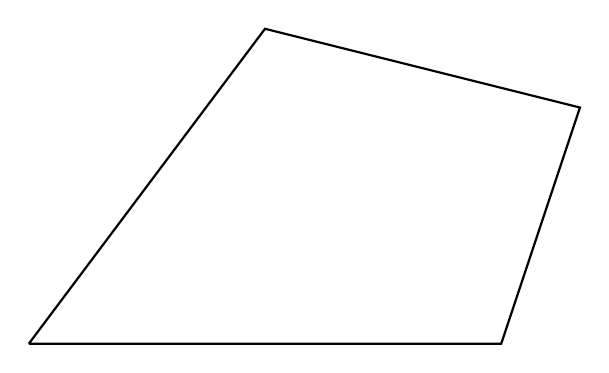
\begin{tikzpicture}
        \coordinate (A) at (0, 0);
        \coordinate (B) at (3, 4);
        \coordinate (C) at (7, 3);
        \coordinate (D) at (6, 0);

        \coordinate (MAB) at (1.5, 2);
        \coordinate (B) at (3, 4);
        \coordinate (C) at (7, 3);
        \coordinate (D) at (6, 0);

        \draw[thick] (A) --  (B) -- (C) -- (D) -- (A);

    \end{tikzpicture}
\end{figure}
